\chapter{Conexión por caminos}%
\label{cha:conexion_por_caminos}
\begin{defi}
Un \underline{camino} en un espacio $X$ es una aplicación continua $\alpha: \left[ a, b \right] \subset \mathbb{R}_u \rightarrow X$. Decimos:
\begin{itemize}
    \item $\alpha$ \underline{va de} $\alpha\left( a \right)$ a $\alpha\left( b \right)$, \underline{conecta} $\alpha\left( a \right)$ con $\alpha\left( b \right)$, que son \underline{extremos}.
    \item La imagen $\alpha\left[ a, b \right] \subset X$ es la \underline{traza}, conexa por imagen continua.
\end{itemize}
\end{defi}

\begin{prop}[Cambios de parámetros]
$\forall \varphi: \left[ c, d \right] \rightarrow \left[ a, b \right]$ continua $\Rightarrow \beta = \alpha \circ \varphi$ es otro camino con igual traza.    

$\varphi$ es un \underline{cambio de parámetro} cuando es homeomorfismo (creciente o decreciente).
%TODO: Imagen
\begin{center}
    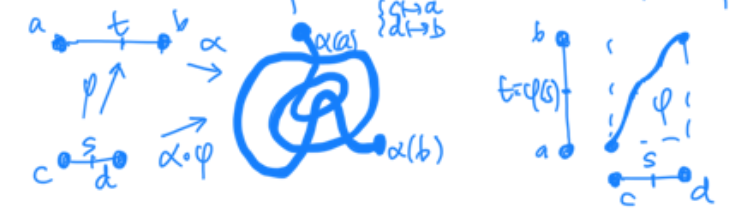
\includegraphics[scale=0.3]{images/camb_par_caminos} 
\end{center}
\end{prop}

\begin{ej}[Interpolación lineal]
Dados $p, q \in \mathbb{R}^n,\ \alpha : \left[ 0, 1 \right] \rightarrow \left[ p, q \right]: t \mapsto \left( 1 - t \right) p + tq$ es un camino bien conocido y útil. También sirve para reparametrizar si $\left[ p, q \right] = \left[ a, b \right] \subset \mathbb{R}$. Vemos, por ejemplo, que siempre podemos reducirnos a caminos con dominio $\left[ 0, 1 \right]$. Esto será fundamental más adelante. 
\end{ej}

\begin{prop}[Producto de caminos]
Topológicamente: 
%TODO: Imagen
\begin{center}
    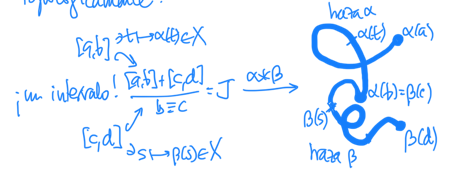
\includegraphics[scale=0.3]{images/prod_caminos} 
\end{center}
(Alternativa: Reparametrizar $\beta$ con dominio $\left[ b, b + \left( d - c \right) \right]$)
\end{prop}

\begin{ej}
Si hacemos el producto de segmentos consecutivos obtenemos \underline{caminos poligonales}. 
\end{ej}

\section{Conexión por caminos}%
\label{sec:conexion_por_caminos}
\begin{defi}
Un espacio $X$ es \underline{conexo por caminos} si sus puntos se pueden conectar con un camino:
\[
\forall x \forall y \in X,\ \exists \sigma_y: \left[ a, b \right] \rightarrow X,\ \sigma_y\left( a \right) = x\; \land \;\sigma_y\left( b \right) = y
\]
En particular, $X = \bigcup_{y} \sigma_y\left[ a, b \right]$ es \underline{conexo} (pivote, $\alpha_y\left( a \right) = x,\ \forall y$)
\end{defi}

\begin{ej}
\begin{enumerate}
    \item La mayor parte de los conexos conocidos son conexos por caminos:
    \begin{itemize}
        \item Los abiertos conexos (top. Usual) son conexos por poligonales, que son caminos.
        \item Los conjuntos convexos y los estrellados también.
    \end{itemize}
    \item El seno del topólogo $\Gamma$ es la traza de $\alpha\left( t \right) = \left( t, \sin\frac{1}{t} \right),\ t > 0$, es conexo y lo es su adherencia $\overline{\Gamma} = J \cup \Gamma,\ J = \{0\} \times \left[ 0, 1 \right]$. Pero $\overline{\Gamma}$ \underline{no} es conexo por caminos.
    \begin{demo}
        No existen caminos $\sigma: \left[ a, b \right] \rightarrow \overline{\Gamma} \begin{cases}
            \sigma\left( a \right) = p \in J\\
            \sigma\left( b \right) = q \in \Gamma
        \end{cases}$:
        \begin{center}
            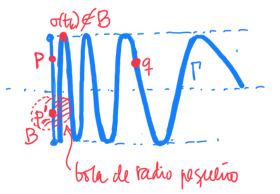
\includegraphics[scale=0.3]{images/dem_sin_top_no_conx_caminos} 
        \end{center}
        \begin{enumerate}
            \item $\sigma\left( t \right) = \left( \alpha\left( t \right), \beta\left( t \right) \right),\ \alpha, \beta$ continuas. $\exists a' = \max \{t \in \left[ a, b \right] : \alpha\left( t \right) = 0\} \Rightarrow (\alpha$ continua en un compacto) %TODO: Fix orden 
            $\Rightarrow \begin{cases}
                \alpha\left( a' \right) = 0,\ \sigma\left( a' \right) = p' \in J\\
                t > a': \alpha\left( t \right) > 0 \Rightarrow \sigma\left( t \right) \in \Gamma \Rightarrow \beta\left( t \right) = \sin \frac{1}{\alpha\left( t \right)} 
            \end{cases} $

            \item Supongamos $p' = \sigma\left( a' \right) \neq \left( 0, 1 \right)$ y $\exists \delta: B\left( p', \delta \right) \cap \{y = 1\} = \emptyset$. $\sigma$ continua $\Rightarrow \exists \sigma\left[ a', \varepsilon \right] \subset B\left( p', \delta \right) \Rightarrow \sigma\left[ a', \varepsilon \right] \cap \{y = 1\} = \emptyset$. (si $p' = \left( 0, 1 \right)$ evitariamos? $\{y = -1\}$)

            \item $\alpha$ continua $\Rightarrow \alpha\left[ a', \varepsilon \right] \subset \mathbb{R}$ conexo compacto $=$ intervalo: $\alpha\left[ a', \varepsilon \right] = \left[ 0, c \right]$.

            \item La oscilación de $\sin \frac{1}{x}$ lleva $\sigma$ a $\{y = 1\}$, fuera de la bola elegida:
            \begin{align*}
            k \gg 0 &\Rightarrow \frac{2}{\left( 1 + 4k \right) \pi} \in \left[ 0, c \right] = \alpha\left[ a', \varepsilon \right] \Rightarrow \exists a' < t_k < \varepsilon: \alpha\left( t_k \right) = \frac{2}{\left( 1 + 4k \right) \pi}\\ 
                &\Rightarrow \sigma\left( t_k \right) = \left( \alpha\left( t_k \right), \sin\left( \frac{1}{\alpha\left( t_k \right)} \right) \right) = \left( x_k, 1 \right) 
            !?\end{align*}
            %TODO: red. abs?
        \end{enumerate}
    \end{demo}
\end{enumerate}
\end{ej}

\section{Mantras}%
\label{sec:mantras_conx_caminos}
Todo (casi) lo que dijimos sobre la conexión nos vale:
\begin{prop}[Mantra del pivote]
    (Igual) Sea $X = \bigcup_{i} A_i,\ \bigcap_{i} A_i \neq \emptyset,\ \forall A_i$ conexos por caminos $\Rightarrow X$ conexo por caminos. 
\end{prop}
\begin{demo}
\begin{center}
    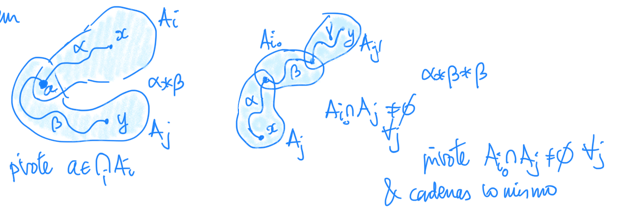
\includegraphics[scale=0.3]{images/dem_pivote_caminos} 
\end{center}
\end{demo}

\begin{prop}[Mantra de la imagen]
Sea $f: X \rightarrow Y$ continua con $X$ conexo por caminos $\Rightarrow f\left( X \right)$ es conexo por caminos. 
\end{prop}
\begin{demo}
\begin{center}
    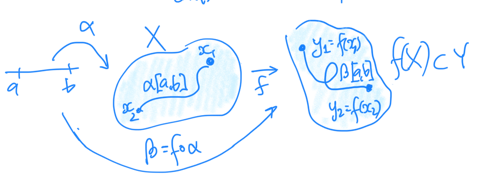
\includegraphics[scale=0.3]{images/dem_imagen_caminos} 
\end{center}
\end{demo}

\begin{prop}[Mantra de la adherencia (¡NO!)]
El seno del topólogo $\Gamma$ = grafo de $\sin \frac{1}{t}$ es conexo por caminos: $\left( a, \sin\frac{1}{a} \right)$ y $\left( b, \sin\frac{1}{b} \right)$ se conectan por el camino evidente, $\alpha\left( t \right) = \left( t, \sin\frac{1}{t} \right),\ a \le t \le b$. Pero, como hemos visto, la adherencia $\overline{\Gamma}$ no es conexa por caminos. 
\end{prop}

\section{Tabla de comportamiento}%
\label{sec:tabla_de_comportamiento_conx_caminos}
%TODO: Fix tabla
\begin{center}    
\begin{tabular}{c | c | c | c | c |}
& Subespacios & Cocientes & Productos & Sumas\\
\hline\\
    Conexión por caminos & $\times$ & \checkmark & \checkmark & $\times$\\
    \hline\\
\end{tabular}
\end{center}

\begin{prop}[Productos]
Sean $\left( x_1, y_1 \right),\ \left( x_2, y_2 \right) \in X \times Y$: 
\[
\begin{rcases}
    \sigma: \left[ a, b \right] \rightarrow X: \begin{cases}
        \sigma\left( a \right) = x_1\\
        \sigma\left( b \right) = x_2
    \end{cases}\\
    \tau: \left[ a, b \right] \rightarrow Y: \begin{cases}
        \tau\left( a \right) = y_1\\
        \tau\left( b \right) = y_2
    \end{cases}
\end{rcases} 
    \Rightarrow \gamma = \left( \sigma, \tau \right) : \left[ a, b \right] \rightarrow X \times Y \begin{cases}
        \gamma\left( a \right) = \left( x_1, y_1 \right)\\
        \gamma\left( b \right) = \left( x_2, y_2 \right)
    \end{cases}  
\]
\end{prop}


\chapter{Componentes conexas\texorpdfstring{\\}{} por caminos y conexión\texorpdfstring{\\}{} local por caminos}%
\label{cha:componentes_conexas_por_caminos_y_conexion_local_por_caminos}
\section{Componentes conexas por caminos}%
\label{sec:componentes_conexas_por_caminos}
Todo análogo a las componentes conexas (casi). Sea $X$ espacio topológico.
\begin{defi}
Una componente conexa por caminos (c.c.c) es un subconjunto conexo por caminos maximal.
\end{defi}
\begin{prop}[Descripción]
\begin{enumerate}
    \item La c.c.c de $x \in X$ es $\bigcup_{x \in A} A$ con $A$ conexa por caminos.
    \item Las c.c.c forman una partición de $X$, más fina que la de las c.c.
    \begin{demo}
        Porque conexo por caminos $\Rightarrow$ conexo pero no la inversa.

        \textbf{¡OJO!} Las c.c.c no son necesariamente cerradas. 

        Como contraejemplo de ambas cosas dichas tenemos la adherencia del seno topólogo. 
    \end{demo}
\end{enumerate} 
\end{prop}

\begin{ej}
    $\Gamma$ seno del topólogo y $\overline{\Gamma} = J \cup \Gamma$ son conexos. Tenemos que $\overline{\Gamma}$ es una c.c, mientras que $J$ y $\Gamma$ son dos c.c.c, una cerrada ($J$) y la otra no ($\Gamma$). [Porque $\overline{\Gamma}$ \underline{no} es conexa por caminos]
\end{ej}

\section{Conexión local por caminos}%
\label{sec:conexion_local_por_caminos}
Imitamos sin sorpresa las demostraciones de la conexión local y tenemos:
\begin{defi}
$X$ es \underline{localmente conexo por caminos} si $\forall x \in X,\ \exists \mathcal{B}^x$ base de entornos abiertos conexos por caminos.
\end{defi}
\begin{prop}
$X$ es localmente conexo por caminos $\Leftrightarrow$ c.c.c de un abierto es abierto.
\end{prop}

\underline{Ejercicio}:
Locamente conexo $\Leftrightarrow \forall x \in X,\ \exists \mathcal{V}^x$ base de entornos conexos por caminos. 

\section{Tabla de comportamiento}%
\label{sec:tabla_de_comportamiento_conx_local_caminos}
%TODO: Fix tabla
\begin{center}    
\begin{tabular}{c | c | c | c | c |}
& Subespacios & Cocientes & Productos & Sumas\\
\hline\\
    Conexión local por caminos & $\times$ & \checkmark & \checkmark & \checkmark\\
    \hline\\
\end{tabular}

También vale que las c.c.c del producto son los productos de las c.c.c de los factores.
\end{center}

\section{Relaciones entre las propiedades de conexión}%
\label{sec:relaciones_entre_las_propiedades_de_conexion}
Lo principal es que:
\begin{prop}
Conexo y localmente conexo por caminos $\Rightarrow$ Conexo por caminos.
\end{prop}
\begin{demo}
\begin{itemize}
    \item Conexo $\Rightarrow \forall x, y,\ \exists \text{ cadenas de } x \text{ a } y$.
    \item Localmente conexo por caminos $\Rightarrow$ cadenas de abiertos conexos por caminos $\Rightarrow{\text{Var. pivote}}$ Estas cadenas son conexas por caminos.
\end{itemize}
Por tanto, $\exists$ camino de $x$ a $y$.
\end{demo}
\begin{obs}
    Esta es la demostración de que un abierto conexo de $\mathbb{R}_u^n$ lo es por poligonales (se usan cadenas de bolas).
\end{obs}

\begin{obs}[Resumen]
Por especificar todas las posibilidades:
%TODO: Imagen
\begin{center}
    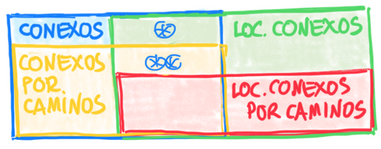
\includegraphics[scale=0.3]{images/resumen_conx} 
\end{center}
\end{obs}

\underline{Ejercicio}: Contraejemplos. Los menos fáciles son $*$ y $**$ 
